% ====================================================================
% PHYSICS TRACK
% ====================================================================
\chapter{Binary Cahn--Hilliard: two free energies}
\label{ch:p1}

\begin{keybox}
\textbf{Key idea.} A blend of two components lowers its free energy by
\emph{demixing}. The Cahn--Hilliard equation is the conserved gradient
flow of a Ginzburg--Landau free energy; that free energy can only
decrease in time, and it splits into a \emph{bulk} (mixing) part and an
\emph{interfacial} (gradient) part whose competition sets the
morphology and its length scale.
\end{keybox}

\section{The model}

Let $c(\mathbf{x},t)$ be the local volume fraction of one component (a
\emph{conserved} order parameter: the total amount of each species is
fixed). The Ginzburg--Landau free energy is
%
\begin{equation}
  F[c] \;=\; \intv \Big[\, f(c) \;+\; \tfrac{\kappa}{2}\,|\grad c|^2 \,\Big]\,dV ,
  \label{eq:F}
\end{equation}
%
with two contributions:
\begin{itemize}[nosep]
  \item the \textbf{bulk} (homogeneous) free energy density $f(c)$,
        which is minimized by the pure phases and \emph{penalized} in
        between --- this is what drives demixing;
  \item the \textbf{interfacial} term $\tfrac{\kappa}{2}|\grad c|^2$,
        which penalizes spatial variation of $c$ and therefore
        \emph{opposes} demixing at short scales. The coefficient
        $\kappa>0$ has units of energy$\times$length$^2$ and sets the
        interface width $\ell \sim \sqrt{\kappa}$.
\end{itemize}

Because $c$ is conserved, the dynamics is the \emph{conserved}
(Model-B) gradient flow of \eqref{eq:F}: mass moves down gradients of
the chemical potential $\mu = \delta F/\delta c$,
%
\begin{equation}
  \dd{c}{t} = \grad\!\cdot\!\big(M\,\grad\mu\big),
  \qquad
  \mu = f'(c) - \kappa\,\grad^2 c .
  \label{eq:ch}
\end{equation}
%
Here $M>0$ is the mobility (how fast mass responds to a chemical-potential
gradient; it sets the \emph{time} scale but not the equilibrium
morphology). The fourth-order PDE is split into the two second-order
equations \eqref{eq:ch} --- the \emph{mixed} $(c,\mu)$ form the solver
uses.

\begin{keybox}
\textbf{$F$ is a Lyapunov functional.} Taking $dF/dt$ along
\eqref{eq:ch} and integrating by parts with no-flux boundaries gives
$\;dF/dt = -\!\intv M\,|\grad\mu|^2\,dV \le 0$. The free energy can
only decrease. Watching it decrease --- and split between bulk and
interface --- is how you \emph{see} the physics in the numbers.
\end{keybox}

\section{Two bulk free energies}

\paragraph{Polynomial double well (the canonical model).}
The simplest $f$ with two equal minima,
%
\begin{equation}
  f_{\text{poly}}(c) = \tfrac14\,(c^2-1)^2,\qquad
  f'=c^3-c,\qquad f''=3c^2-1,\qquad c\in[-1,1].
\end{equation}
%
The two phases are $c=\pm1$; the region $f''<0$ (i.e. $|c|<1/\sqrt3$)
is \emph{spinodally unstable} --- any small fluctuation there grows.
This model is dimensionless and symmetric; it isolates the phase-field
mechanism from material detail.

\paragraph{Flory--Huggins (the physical model).}
For a real blend the mixing free energy is entropic $+$ enthalpic,
%
\begin{equation}
  f_{\text{fh}}(c) = A\,\big[c\ln c + (1-c)\ln(1-c)\big] + B\,c(1-c),
  \qquad c\in(0,1),
  \label{eq:fh}
\end{equation}
%
where the logarithmic \emph{entropy of mixing} (scale $A\sim 1/N$, with
$N$ the degree of polymerization) always favors mixing, and the
\emph{enthalpic} term $B\,c(1-c)$ (with $B$ the Flory interaction
parameter $\chi$) favors demixing when the components dislike each
other. The curvature
%
\begin{equation}
  f_{\text{fh}}''(c) = A\Big(\tfrac1c + \tfrac1{1-c}\Big) - 2B
\end{equation}
%
is negative --- unstable --- only where the enthalpic $-2B$ beats the
(always convex) entropic term. This is the \emph{spinodal}. The logs
diverge at the pure phases, so Flory--Huggins keeps $c$ strictly inside
$(0,1)$ (no unphysical overshoot), at the cost of a stiff $f''$ near
the walls --- a numerical point we return to in the Computational
track.

\begin{keybox}
\textbf{Coefficients and their ranges.}
$M>0$ (mobility, time scale). $\kappa>0$ (gradient penalty; interface
width $\sqrt\kappa$ --- choose it so the interface spans $\sim$3--5 mesh
cells). Polynomial: no free parameters. Flory--Huggins: $A>0$
(entropy, $\sim1/N$; $A\to0$ for long polymers), $B=\chi$ (interaction;
demixing requires $B$ large enough that $f''<0$ somewhere ---
for $A=1$ the symmetric point $c=\tfrac12$ is unstable once $B>2A=2$).
The tutorial uses $A=\FHA$, $B=\FHB$ (a clear quench); real blends map
$A\sim1/N$, $B\sim\chi$ (see \file{materials/materials.yaml}).
\end{keybox}

\section{Run it}

\begin{runbox}
\textbf{Run it.}
\begin{lstlisting}
cd physics/01_ch_binary_energies
python run.py            # both free energies, 128x128
\end{lstlisting}
It marches a spinodal decomposition from a nearly uniform blend
($c=\bar c + $ small noise) for both free energies, printing the energy
budget. Compare the printed table with \file{EXPECTED.md} and the
figures below.
\end{runbox}

\paragraph{What you should see.}
From a nearly uniform, slightly noisy blend, small fluctuations in the
unstable region grow (spinodal decomposition), sharpen into domains
separated by thin interfaces, and then \emph{coarsen}. The total free
energy drops monotonically (after a one-step start-up transient
discussed below), mass is conserved to solver tolerance, and the field
saturates at the two coexisting phases.

% --- generated by gen_figures.py ---
\begin{figure}[h]\centering
  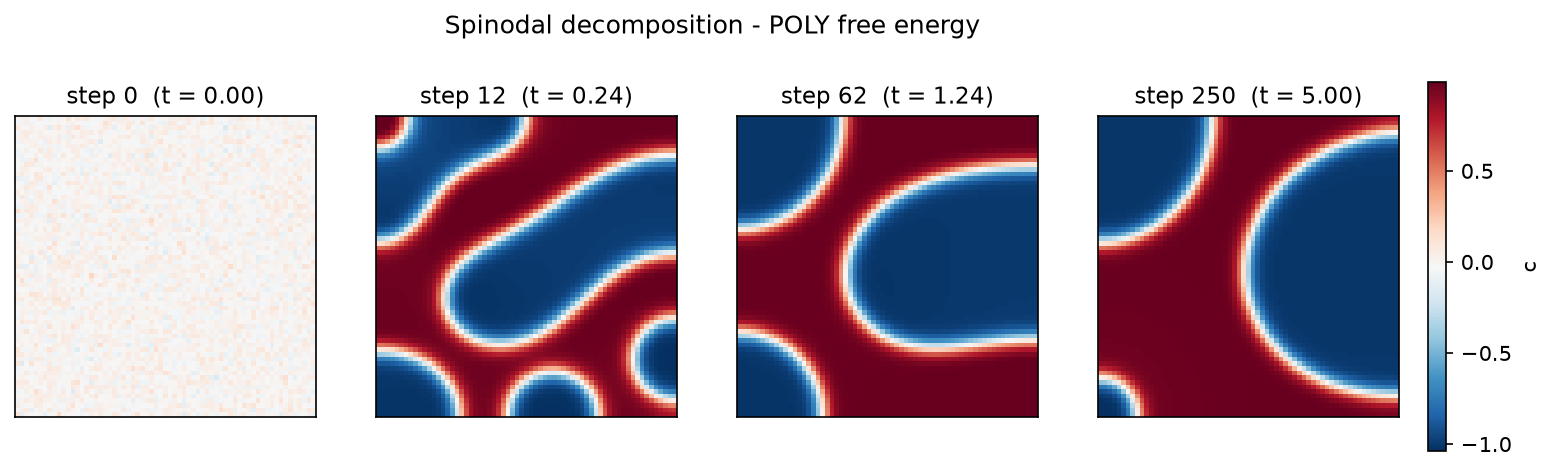
\includegraphics[width=\linewidth]{figures/p1_morph_poly.png}\\[4pt]
  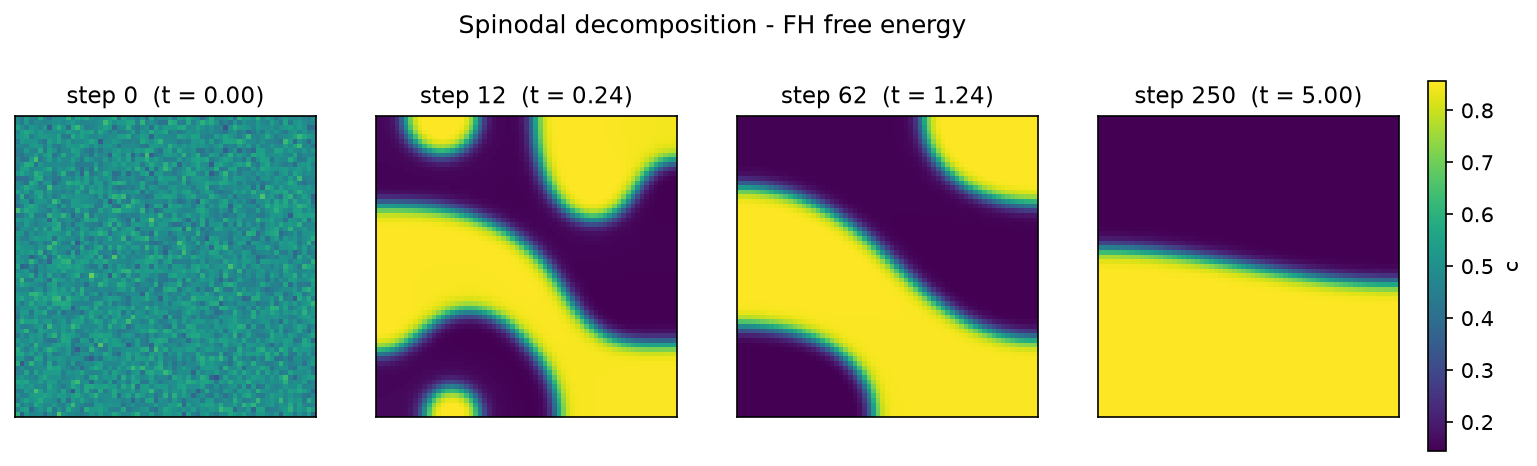
\includegraphics[width=\linewidth]{figures/p1_morph_fh.png}
  \caption{Spinodal decomposition and coarsening for the polynomial
    (top, $c\in[-1,1]$) and Flory--Huggins (bottom, $c\in(0,1)$) free
    energies, at the mesh and parameters of the tutorial. Same mixing
    physics, different order-parameter range and interface structure.}
  \label{fig:p1morph}
\end{figure}

\begin{figure}[h]\centering
  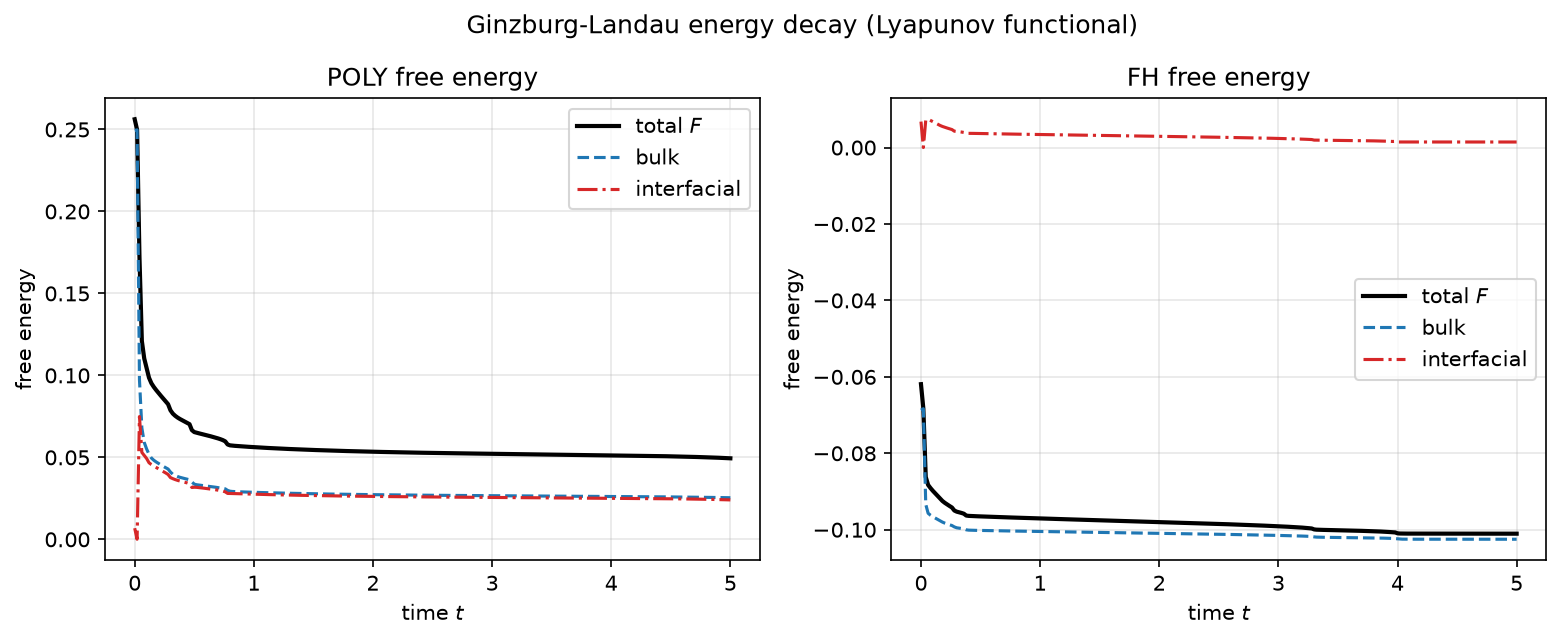
\includegraphics[width=\linewidth]{figures/p1_energy.png}
  \caption{The Ginzburg--Landau energy budget: total free energy (black)
    and its bulk (blue) and interfacial (red) parts versus time. The
    total is a Lyapunov functional --- monotone decreasing. Early on,
    forming interfaces \emph{raises} the interfacial energy while the
    bulk energy falls faster; during coarsening, domains merge and the
    interfacial energy falls as total interface area shrinks.}
  \label{fig:p1energy}
\end{figure}

\begin{keybox}
\textbf{Measured self-check} (your \file{run.py} should reproduce
these to a few significant figures; exact values depend on the RNG seed
fixed in the tutorial).
\begin{center}\small
\begin{tabular}{lcc}
\toprule
 & polynomial & Flory--Huggins \\
\midrule
total $F$: start $\to$ end       & \POLYFstart\ $\to$ \POLYFend & \FHFstart\ $\to$ \FHFend \\
interfacial energy: peak $\to$ end & \POLYFintpeak\ $\to$ \POLYFintend & \FHFintpeak\ $\to$ \FHFintend \\
phase values $[c_{\min},c_{\max}]$ & \POLYcrange & \FHcrange \\
mass drift $|\Delta m|$           & \POLYmass & \FHmass \\
$F$ monotone after step 1         & yes & yes \\
\bottomrule
\end{tabular}
\end{center}
\end{keybox}

\section{Code walk-through}

The tutorial's physics lives in \file{spinodal.py}, which drives the
production brick \file{src/diffsim/physics/cahn\_hilliard.py}. The three
sections you interact with:

\paragraph{1. Build a mesh and the stepper.}
\begin{lstlisting}
dm, mesh, cons = build_mesh_dm(level=7, p=1, device="cuda:0")  # 128x128
st = CahnHilliardStepper(dm, M, kappa, dt, order=1,
                         energy="poly")   # or energy="fh"
\end{lstlisting}
\code{energy} selects $f(c)$; \code{order} is the time scheme (1 =
backward Euler); \code{M}, \code{kappa} are the coefficients above. The
constructor is where the \emph{model} is chosen --- everything else is
running it.

\paragraph{2. Seed the initial blend.}
\begin{lstlisting}
st.set_initial(lambda x: c_avg + amp*rng.standard_normal(len(x)),
               mu_init="consistent")
\end{lstlisting}
A nearly uniform field with a small random perturbation --- the seed of
the spinodal instability. \code{mu\_init="consistent"} projects a
matching initial chemical potential so the very first step does not see
an artificial $\mu$-transient (the one-step start-up you see in
Fig.~\ref{fig:p1energy}).

\paragraph{3. March, and measure the energy each step.}
\begin{lstlisting}
for n in range(steps):
    c, mu = st.step()
    F_total, F_bulk, F_int = energy_budget(st, dm, mesh, c, ...)
\end{lstlisting}
\code{step()} advances one time step (assemble $\to$ Newton solve on the
GPU). \code{energy\_budget} evaluates $c$ and $\grad c$ at the Gauss
points --- using the same quadrature the solver uses --- and integrates
the two energy densities of \eqref{eq:F} separately. That is the whole
measurement: no post-processing magic, just the definition of $F$.

\section{Explore on your own}

\question{Vary $\kappa$ over, say, $\{2,5,10\}\times10^{-4}$. How does
the equilibrium interface width scale, and how many mesh cells does the
interface span in each case? At what point do you stop trusting the
result, and why?}

\question{For Flory--Huggins, sweep $B$ (the interaction $\chi$) from
below to above the spinodal threshold $2A$. Where does demixing stop
happening, and does the onset match $f''(\tfrac12)=0$?}

\question{The polynomial model is symmetric ($\bar c=0$); Flory--Huggins
with $\bar c\ne\tfrac12$ is not. Run an off-critical blend
($\bar c=0.35$) and describe how the morphology differs from the
symmetric case (droplets vs.\ bicontinuous). Which blend ratio gives
which?}

\question{The total energy dips monotonically but the interfacial
energy is \emph{non}-monotone. Explain the two regimes (interface
formation vs.\ coarsening) in terms of $F_{\text{bulk}}$ and
$F_{\text{int}}$, and predict how each scales during coarsening.}

\question{Mobility $M$ was said to set the time scale but not the
equilibrium. Test it: double $M$ and check whether the \emph{final}
morphology and energy are unchanged while the \emph{approach} rescales
in time.}
